% For instructions,
\documentclass[reprint, amsmath, amssymb, aps]{revtex4-2}

%\usepackage[norsk]{babel}
%Uncomment this if you want to write in Norwegian

\usepackage{graphicx}% Include figure files
\usepackage{dcolumn}% Align table columns on decimal point
\usepackage{bm}% bold math
\usepackage{hyperref}% add hypertext capabilities
\usepackage{booktabs}
\usepackage{float}
\usepackage{siunitx}



\begin{document}
\title{Project3 - FYS4460}
\author{Mikkel Metzsch Jensen}

\date{\today}
\maketitle
\subsubsection*{1d n(s,p)}
We define the cluster number density $n(s,p)$ as the number of cluster of size $s$ for the system. Thus we have:
\begin{align*}
  \frac{N_s}{L^2}
\end{align*}
where $N_s$ is the number of clusters with size $s$ and $L$ is the dimension of our simulaiton lattice. Hence we can also think of $n(s,p)$ as the probability that a given site is the left-most site in a cluster of size s:
\begin{align*}
  P(\text{site is left-most side of cluster of size s}) = n(s,p)
\end{align*}
(notice the specific choice of the left side is abitrary). For at cluster of size $s$ we can calculate this probability as
\begin{align*}
  n(s,p) = (1-p)p^s(1-p) = (1-p)^2p^s
\end{align*}

% From this we also realize that
% \begin{align*}
%   P(\text{site is part of cluster of size s}) = sn(s,p)
% \end{align*}




\subsection*{f) Estimate n}
We define the cluster number density $n(s,p)$ as
\begin{align*}
  \frac{N_s}{L^2}
\end{align*}
where $N_s$ is the number of clusters with size $s$ and $L$ is the dimension of our simulaiton lattice. Notice that $L^2$ then corresponds to the area. We estimate $n(s,p)$ by performing a number of simulation of a $L\times L$ system and then counting the number of clusters for some intervals of cluster size $s$. Hence we are making a histogram by combinning the data from multiple simulations (Monte Carlo Cycles). Due to the fact that we only have few clusters at higher $s$ spaced for apart one the s-scale, we use logaritmic binning with a binwidth of $a^i$ for bin $i$ to avoid having empty intervals for the histogram. Our estimate $\bar{n(s,p)}$ is calculated as
\begin{align*}
  \bar{n(s,p)} = \frac{N_{s + \Delta s}(M)}{ML^d \Delta s}
\end{align*}
for $M$ simulations, dimension $d$ and binwidth $\Delta_s$. We can then plot $\bar{n(s,p)}$ as a function of $s$. \par
In order to get an intuition for how this will behave, we can use our knowledge of the one-dimensional case. In one dimension we have:
\begin{align*}
  n(s,p) &= (1-p)^2p^s, \quad p_{c,d=1} = 1 \\
  &= (1-p)^2e^{s\ln{(p)}} \\
  &= (1-p)^2 e^{-s/s_\xi}, \quad s_\xi=-\frac{1}{\ln{(p)}}
\end{align*}
Where we have introduced $s_{\xi}$ which by our definition appears to be some charecteristic cluster size. When $s = s_\xi$ $n(s,p)$ have dropped to $1/e$ and when $s \gg s_\xi$ we have $n(s,p)=0$. From the definition of $s_\xi$ we see that it diverges for $p \to 1$ which corresponds well of the expectation that the charecteristic cluster size will diverge as it transistions to spanning the infinte plane. We then study the case $1-p \ll 1 \Longleftrightarrow p \approx 1$.
\begin{align*}
  \ln{(p)} = \ln{(1 - (1-p))} = - (1-p)
\end{align*}
where we used the taylor expansion $ln{(1+x)} \approx x$ for $x \ll 1$. We can then rewrite $s_\xi$ as
\begin{align*}
  s_\xi = -\frac{1}{\ln{(p)}} \approx \frac{1}{p-1} = \frac{1}{p_c -p}, \quad p_c-p << 1
\end{align*}
We shall se that it is usefull to introduce the exponent $\sigma$ such that
\begin{align*}
  s_\xi = \frac{1}{(p_c -p)^{1/\sigma}}
\end{align*}
where $\sigma = 1$ for one dimension. When $p \to p_c$ we have $s_\xi \to \infty$. By using the one dimensional case we can do as follows
\begin{align*}
  N(s,p) &= (1-p)^2e^{-s/s_\xi},  \\
  &= (p_c - p)^2 e^{-s/s_\xi} \\
  &= s_\xi^{-2} e^{-s/s_\xi} \\
  &= \left(\frac{s}{s_\xi}\right)^2s^{-2} e^{-s/s_\xi} \\
  &= s^{-2} \left[\left(\frac{s}{s_\xi}\right)^2e^{-s/s_\xi}\right]
\end{align*}
We get an area where $s < s_\xi$ where the first term dominates and this $n(s,p)$ is only dependent on $s$ and then when $s \ge s_\xi$ the second term dominates and becomes dependent of $s_\xi$. \par This motivates the scaling ansatz
\begin{align}
  n(s,p) = s^\tau F\left(\frac{s}{s_\xi}\right), \quad s_\xi \propto |p-p_c|^{-1/\sigma}
  \label{eq:scaling_ansatz}
\end{align}
where $F(s/s\xi)$ should have some exponential decay. Notice that this ansatz is also motivated by the analytical results of the system in infinte dimensions. \par
We will know investegate this for two dimension. We begin by plotting $n(s,p)$ as a function of $s$ on a log10 plot when approaching $p_c$ from below. We use the exact value of $p_c = 0.59275$ (found by numerical study) for now, but we will estimate our own value for this later on. The result is shown in figure c

\begin{figure}[H]
  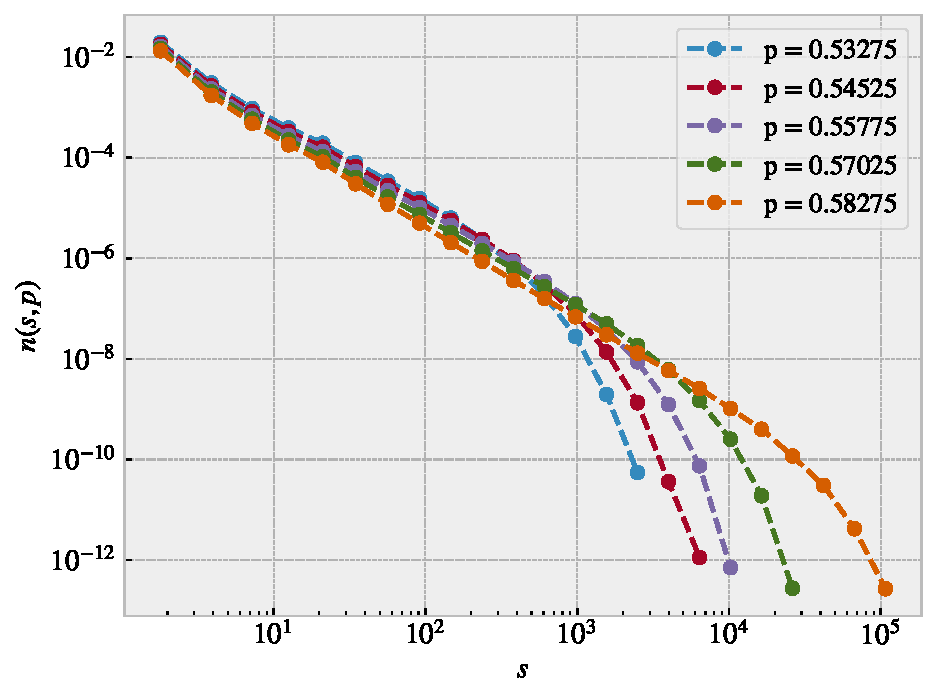
\includegraphics[width=\linewidth]{figures/f_p_below.pdf}
  \caption{$n(s,p)$ with $p$ approaching $p_c = 0.59275$ from below in a $L \times L = 1000 \times 1000$ system. The results are averaged over 300 Monte Carlo cycles with a logaritmic binsize of $1.6^i$ for bin $i$.}
  \label{fig:f_below}
\end{figure}

One the log plots we see a linear section corresponding to the expected $ s^\tau$ and then for higher $s$ a seciton where $n(s,p)$ drops fast correesponding to the expected contribution from $F\left(\frac{s}{s_\xi}\right)$. We also take a look at this relation when approaching $p_c$ from above shown in figure \ref{fig:f_above}

\begin{figure}[H]
  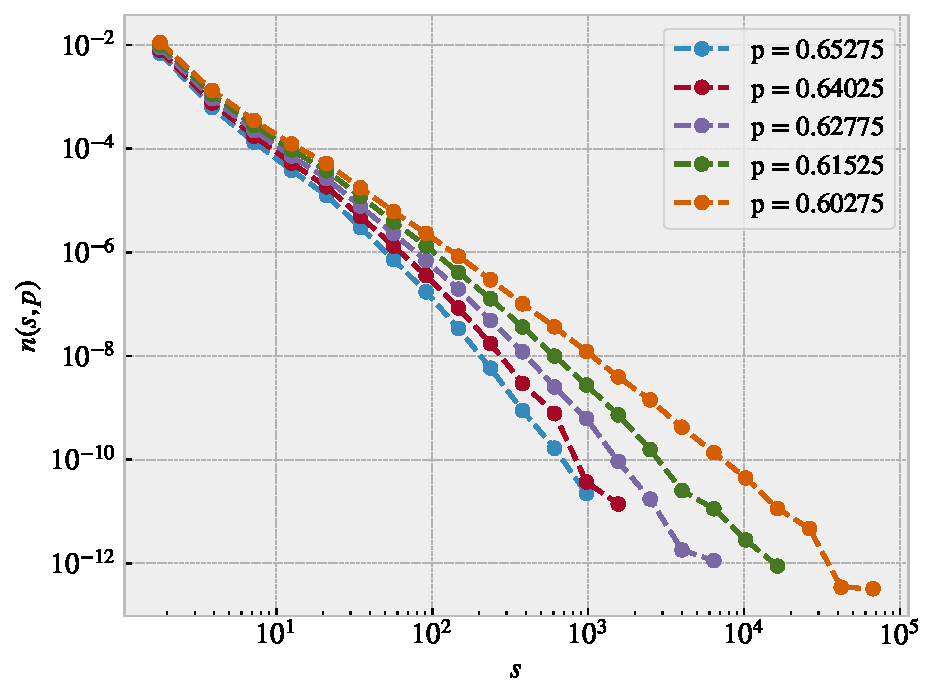
\includegraphics[width=\linewidth]{figures/f_p_above.pdf}
  \caption{$n(s,p)$ with $p$ approaching $p_c = 0.59275$ from above in a $L \times L = 1000 \times 1000$ system. The results are averaged over 300 Monte Carlo cycles with a logaritmic binsize of $1.6^i$ for bin $i$.}
  \label{fig:f_above}
\end{figure}

We see some similar trends on figure \ref{fig:f_above} as \ref{fig:f_below}, but it does not match entirely.
%
%%
%%%
%%
%
\subsection*{g)}
We know investegate $n(s,p)$ as a function of size $L$ at $p=p_c$. By the use of the scaling ansatz \ref{eq:scaling_ansatz} we expect a linear trend with slope $-\tau$ for $s<s_\xi$ when using a logaritmic plot. We simulate systems with $L = 2^k$ for $k = [4,9]$ and determine $\tau$ as linear fit on the logaritmic plot for the biggest value of $L$. The results is shown in figure \ref{fig:g}.

\begin{figure}[H]
  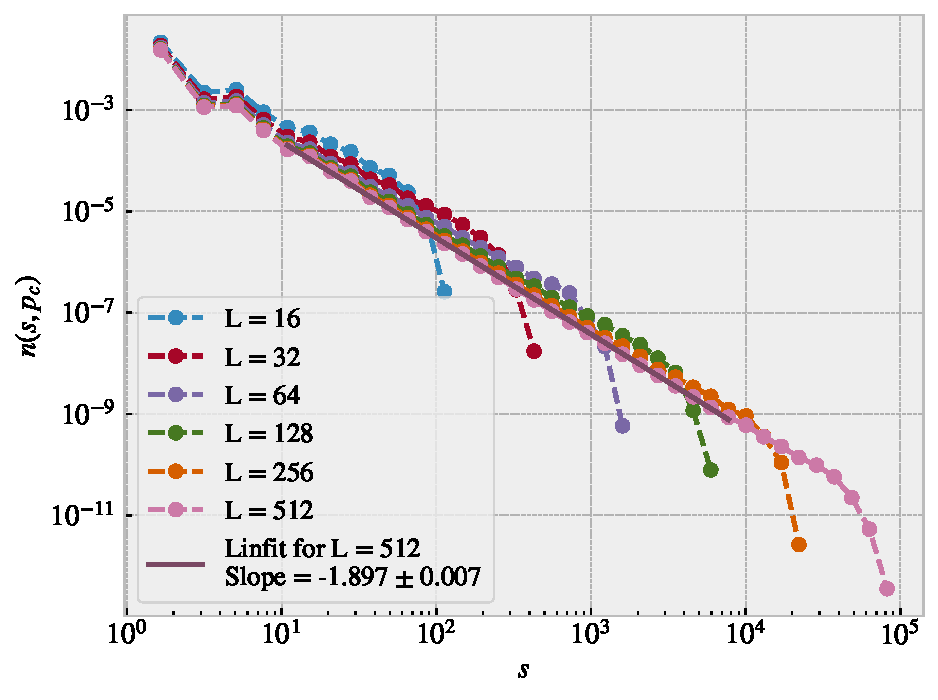
\includegraphics[width=\linewidth]{figures/g.pdf}
  \caption{$n(s,p)$ with $p = p_c = 0.59275$ with $L = 2^k$ for $k = 4, \cdots, 9$ The results are averaged over 1000 Monte Carlo cycles with a logaritmic binsize of $1.1^i$ for bin $i$. By making a linear fit on the first part of the datapoints for $L = 512$ we estimate $\tau$ as $1.89$.}
  \label{fig:g}
\end{figure}
On figure \ref{fig:g} we see as predicted a good linear fit for lower value of $s$. The point for which the function $F\left(\frac{s}{s_\xi}\right)$ begin to domniate the trend (where $s > s_\xi$) is clearly effected by the choice of L. When the system size is increased the transisiton point moves towards higer values of $s$. \par
The given estimate for $\tau$ according to \cite{textbook} is $\tau = 187/91 \approx 2.05$ giving a relative error of
\begin{align*}
  \eta_\tau= \left|\frac{187/91 - 1.89}{187/91}\right| = 0.080
\end{align*}
%
%%
%%%
%%
%
\subsection*{h)}
We know want to esitmate the of $s_\xi$. From the scaling ansatz we define this be the place where the function $F\left(\frac{s}{s_\xi}\right)$ start to dominate. Thus we define $s_\xi$ as the point where the values for $n(s,p)$ have dropped to half of that following the $s^{-\tau}$ relation. Hence we use the following definition of $s_\xi$:
\begin{align*}
  \frac{n(s,p)}{n(s,p_c)} = \left(\frac{s}{s_\xi}\right) = 0.5
\end{align*}
By plotting the fraction $n(s,p)/n(s,p_c)$ against $s$ on a logaritmic plot and finding the interception (using interpolation) between the slopes and the line $n(s,p)/n(s,p_c) = 0.5 $ we can dtermine estimates for $s_\xi$ at different probabilites $p$. This is showecased for a selection of probabilities in figure \ref{fig:h_n_over_nc.pdf}
\begin{figure}[H]
  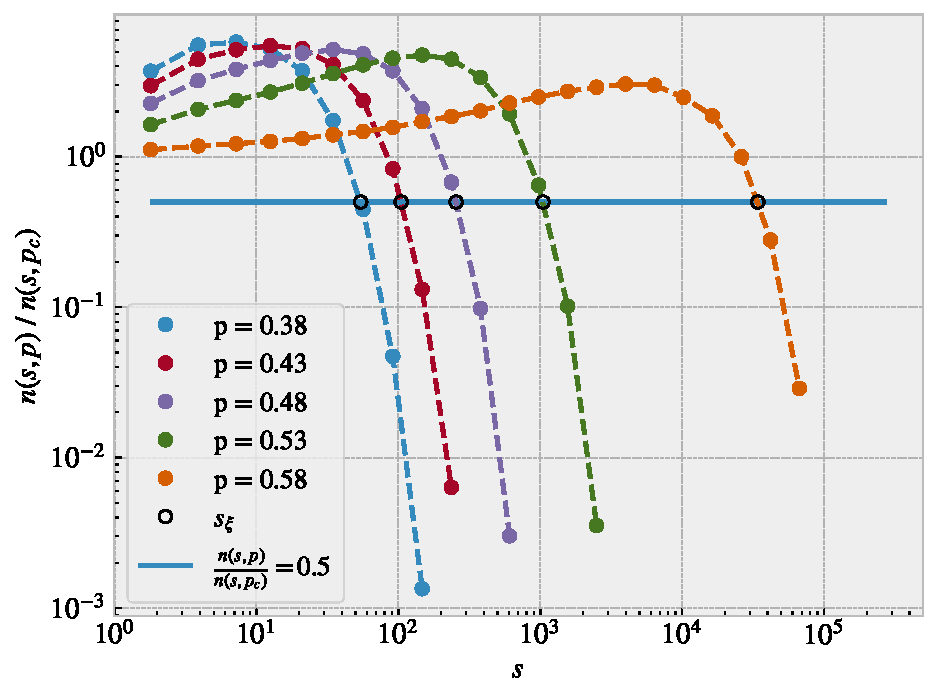
\includegraphics[width=\linewidth]{figures/h_n_over_nc.pdf}
  \caption{L = 1000, MC = 500, a = 1.6}
  \label{fig:h_n_over_nc.pdf}
\end{figure}
Following the scaling ansatz we expect $s_\xi \sim |p-p_c|^{-1/\sigma}$ and thus we can estimate $\sigma$ as the negative inerse slope on a logaritmic plot of $s_\xi$ against the difference $|p-p_c|$. This is shown in figure \ref{fig:h} for 20 values of $p \in [0.56, 0.58]$.
\begin{figure}[H]
  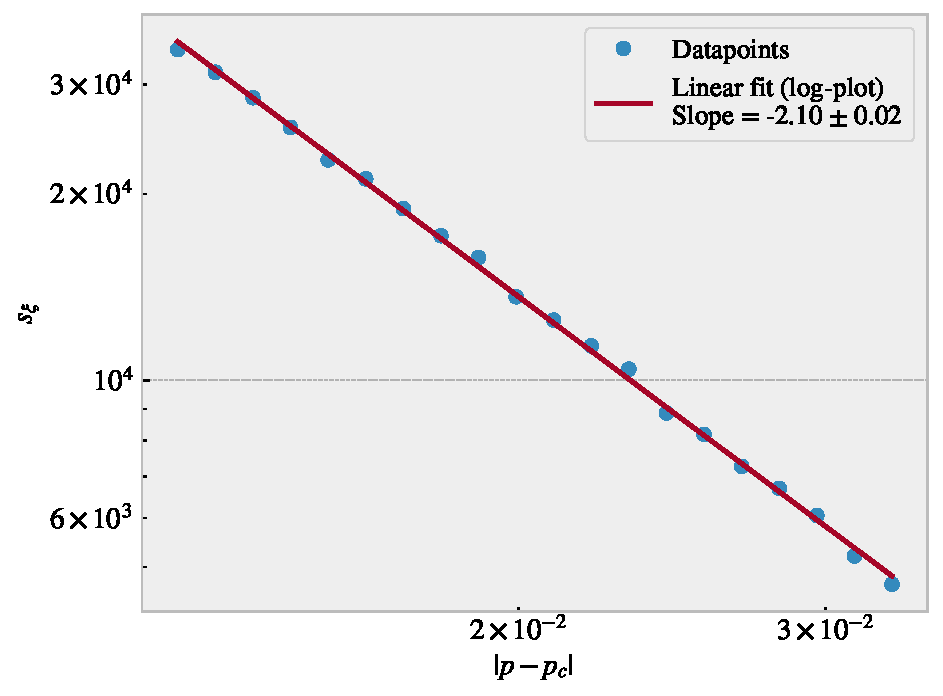
\includegraphics[width=\linewidth]{figures/h_sigma.pdf}
  \caption{$s_{\xi}$ defined as $n(s,p)/n(s,p_c) = F(s/s_{\xi}) = 0.5$ as a function of $|p-p_c|$ for 20 equally distributed values in the interval $p \in [0.56, 0.58]$. For each value of $p$ we used a system size of $L = 1000$, a logaritmic binsize of $1.6^i$ for bin $i$ and averagede the result for 500 MC cycles. Notice that choosing $0.58 < p \le p_c$ gave more unreliable results as the relations diverges near $p_c$}
  \label{fig:h}
\end{figure}
From the linear fit on \ref{fig:h} we find
\begin{align*}
  \sigma = -\frac{1}{\text{slope}} =  0.475 \pm 0.004
\end{align*}
The given estimate for $\sigma$ according to \cite{textbook} is $\sigma = 36/91 \approx 0.40$ giving a relative error
\begin{align*}
  \eta_\sigma = \left|\frac{36/91 - 0.48}{36/91}\right| = 0.21
\end{align*}
%
%%
%%%
%%
%
\subsection*{i)}
Handles multiple spanning cluster by mean value.
\begin{figure}[H]
  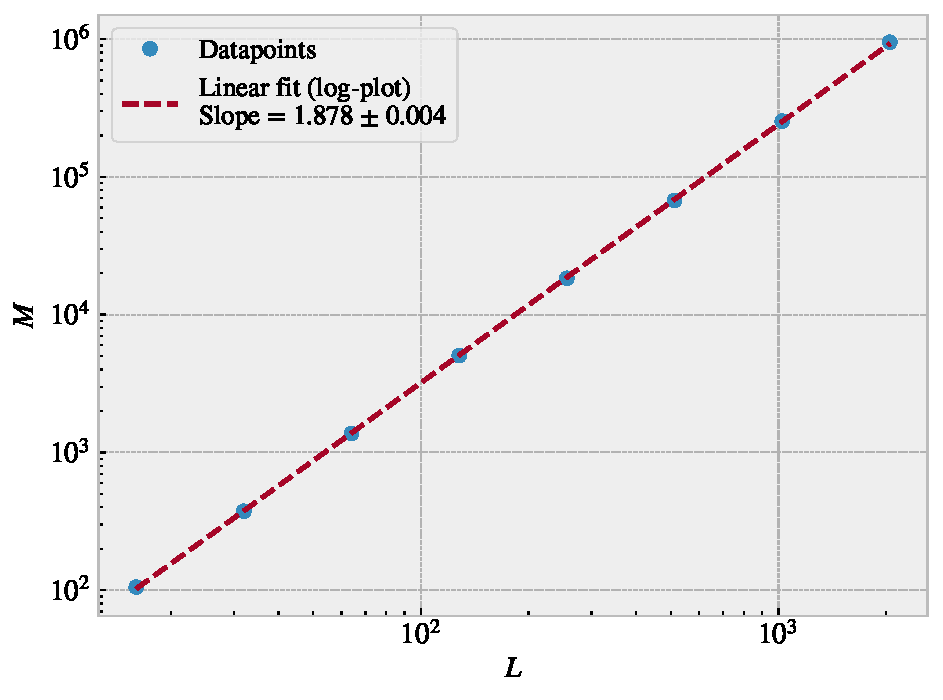
\includegraphics[width=\linewidth]{figures/i.pdf}
  \caption{$MC_cycles = 500$}
  \label{fig:i}
\end{figure}
We find that $M(L)$ goes as
\begin{align*}
  M = L^D, \qquad D = 1.878 \pm 0.03
\end{align*}
The given estimate for $D$ according to \cite{textbook} is
$D = 91/48 \approx 1.896$ giving a relative error
\begin{align*}
  \eta_D= \left|\frac{91/48 - 1.878}{91/48}\right| = 0.009
\end{align*}
%
%%
%%%
%%
%
\subsection*{l)}
We introduce the percolation probability $\Pi(p,L)$ of having a spanning cluster in the system. We can then develop a theory for $\Pi(p,L)$ using finite-size scaling. We take a starting point in the ansatz
\begin{align*}
  P(p,L) = L^x f{\left( \frac{L}{\xi}\right)}
\end{align*}
First consider the limit $p \to p_c$ where we notice from simulations that $\Pi(p,L)$ does not either diverge or go to zero. This means $\Pi(p,L)$ cannot be a function of $\xi$ alone and must have the scaling on form
\begin{align*}
  \Pi(p,L) = L^0f{\left( \frac{L}{\xi}\right)} = f{\left( \frac{L}{\xi}\right)}
\end{align*}
We can rewrite this in terms of $p-p_c$ by inserting $\xi = |p-p_c|^{-\nu}$ which yields
\begin{align*}
  \Pi(p,L) &= f\left(L |p-p_c|^{\nu}\right) \\
  &= f\left(L^{1/\nu} |p-p_c|\right)^\nu
\end{align*}
We introduce a new function $\phi(u) = f\left(u^\nu\right)$ and arrive at the scalling ansatz:
\begin{align}
  \Pi(p,L) = \phi(L^{1/\nu} |p-p_c|)
  \label{eq:SA_Pi}
\end{align}
We then define $p_{\Pi=x}$ such that
\begin{align*}
  \Pi(p_{\Pi = x}) = x
\end{align*}
As $L\to\infty$ we expect any such $p_{\Pi = x}$ to converge towards $p_c$. We notice that $p_{\Pi = x}$ is actually a funciton of $L$. We insert this into the scaling ansatz \ref{eq:SA_Pi}:
\begin{align*}
  x = \phi(L^{1/\nu} |p_{\Pi = x}(L)-p_c|)
\end{align*}
which can be solved as
\begin{align*}
  L^{1/\nu} |p_{\Pi = x}(L)-p_c| = \phi^{-1}(x) = C_x
\end{align*}
where $C_x$ is a number that only depends on $x$ and not $L$. We can therefore rewrite this as
\begin{align}
  |p_{\Pi = x}(L)-p_c| = C_x L^{-1/\nu}
  \label{eq:rel_nu}
\end{align}
This relation can be used determine $\nu$. We simulate a series of system with $L = 25,50,100,200,400,800$ and find $p_{\Pi = x}$ for $x_1=0.3$ and $x_2=0.8$ by interpolation on the estimatet curve for each $\Pi(p,L)$ with 50 values for $p \in [0.4, 0.75]$. The results are shown in figure \ref{fig:l}.
\begin{figure}[H]
  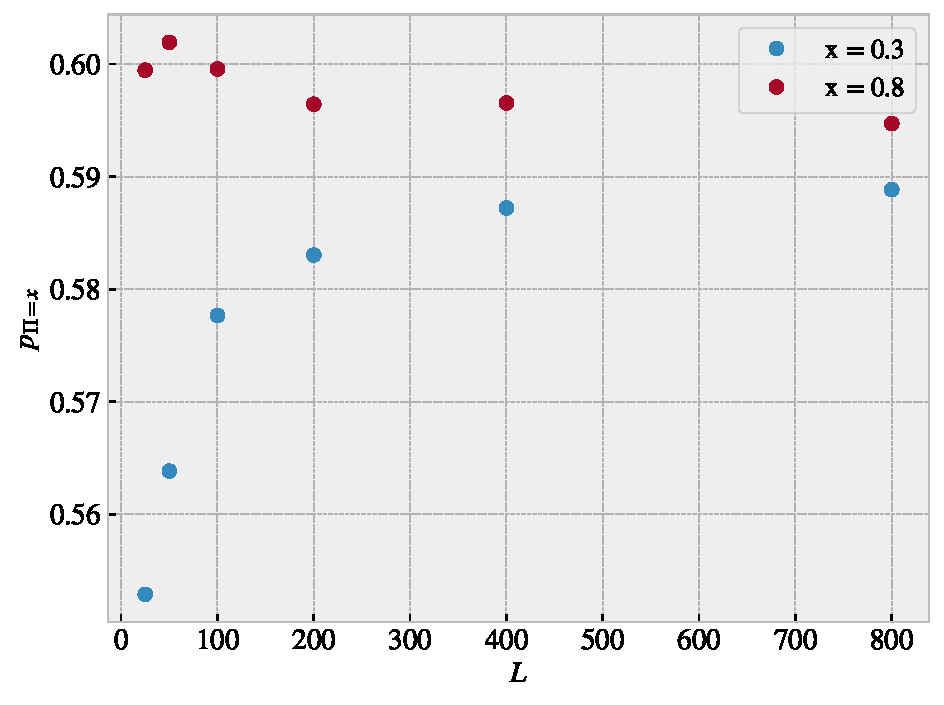
\includegraphics[width=\linewidth]{figures/l.pdf}
  \caption{$p_{\Pi = x}$ as a function of $L$ for $x=0.3$ and $x=0.8$. $p_{\Pi = x}$ is defined through $\Pi(p_{\Pi = x}) = x$ }
  \label{fig:l}
\end{figure}
%
%%
%%%
%%
%
\subsection*{m)}
Frrom \ref{eq:rel_nu} we have
\begin{align*}
  p_{x_1} - p_{x_2} = (C_{x_1} - C_{x_2})L^{-1/\nu}
\end{align*}
We can then plot $\log{(p_{\Pi = 0.8} - p_{\Pi = 0.3})}$ as a function of $\log{(L)}$ to estimate the exponent $\nu$ through the relation
\begin{align*}
  \log{(p_{\Pi = 0.8} - p_{\Pi = 0.3})} =  \log{(C_{x_1} - C_{x_2})} + \log{(L)} \frac{-1}{\nu}
\end{align*}
\begin{figure}[H]
  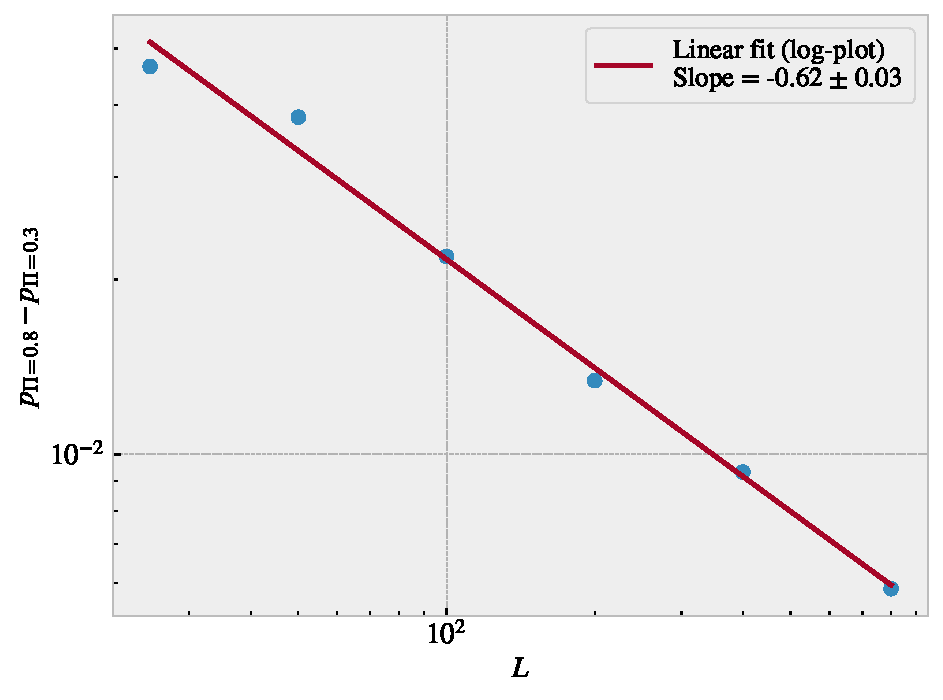
\includegraphics[width=\linewidth]{figures/m.pdf}
  \caption{...}
  \label{fig:m}
\end{figure}
The slope from \ref{fig:m} then coresponds to
\begin{align*}
  \nu = \frac{-1}{\text{slope}} = 1.61 \pm 0.08
\end{align*}
The given estimate for $\nu$ according to \cite{textbook} is $\nu = 4/3 \approx 1.33$ giving a relative error
\begin{align*}
  \eta_\nu= \left|\frac{4/3 - 1.61}{4/3}\right| = 0.208
\end{align*}
%
%%
%%%
%%
%
\subsection*{n)}
In the following we will use the exact value of $\nu = \frac{4}{3}$. From \ref{eq:rel_nu} we have (should be fine with absolute values when adressing this properly)
\begin{align*}
  p_{\Pi=x} = p_c + C_xL^{-1/\nu}
\end{align*}
We can then estimate $p_c$ as the intersection of the linear fit for $p_{\Pi=x}$ as a function of $L^{-1/\nu}$
\begin{figure}[H]
  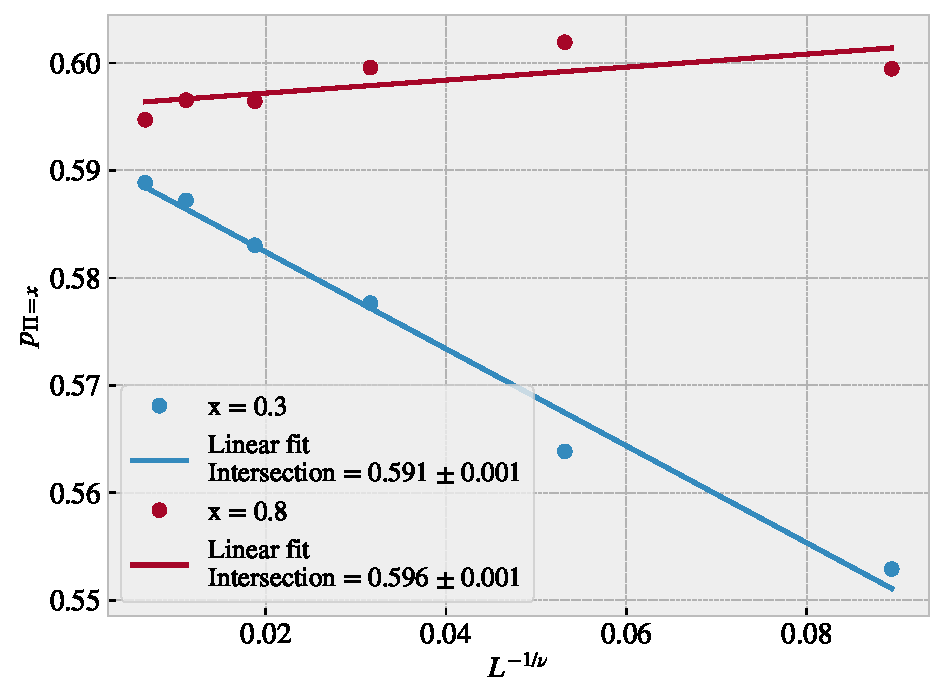
\includegraphics[width=\linewidth]{figures/n.pdf}
  \caption{...}
  \label{fig:n}
\end{figure}
From the results on figure\ref{fig:n} we estimate
\begin{align*}
  p_c = 0.594 \pm 0.002
\end{align*}
The given estimate for $p_c$ according to \cite{textbook} is $p_c = 0.59275$ giving a relative error
\begin{align*}
  \eta_\nu= \left|\frac{0.59275 - 0.594}{0.59275}\right| = 0.0021
\end{align*}
From this we can find the function $\phi(u)$ by plotting $\Pi$ against $L^{1/\nu}(p-p_c)$. This is showed in figure \ref{fig:n2}
\begin{figure}[H]
  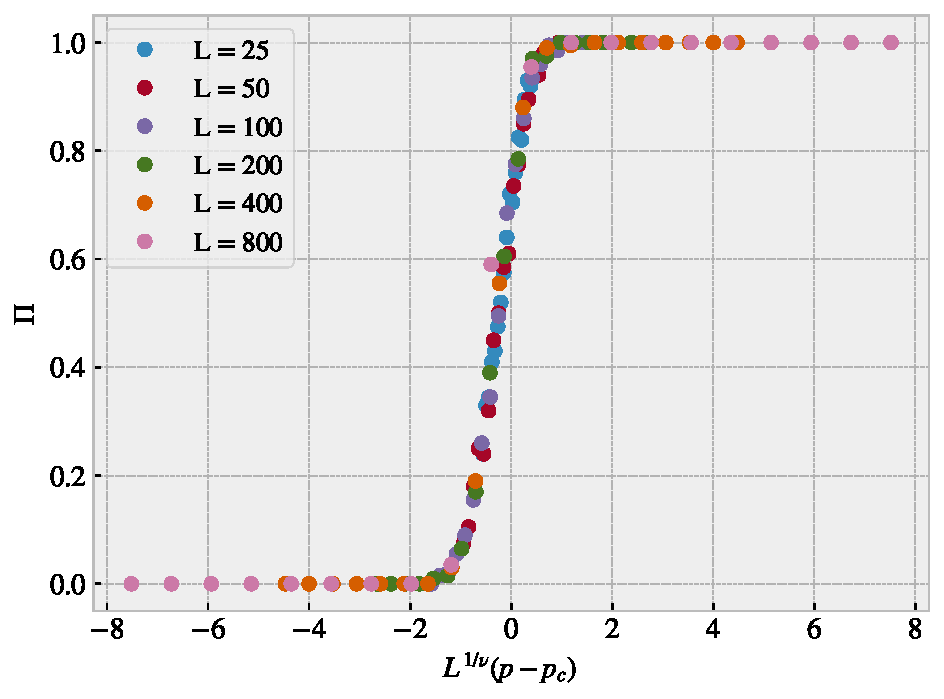
\includegraphics[width=\linewidth]{figures/n2.pdf}
  \caption{...}
  \label{fig:n2}
\end{figure}
%
%%
%%%
%%
%
\subsection*{q)}
Making assumption
\begin{align*}
  M_{SC} \propto L^{D_{SC}}
\end{align*}
\begin{figure}[H]
  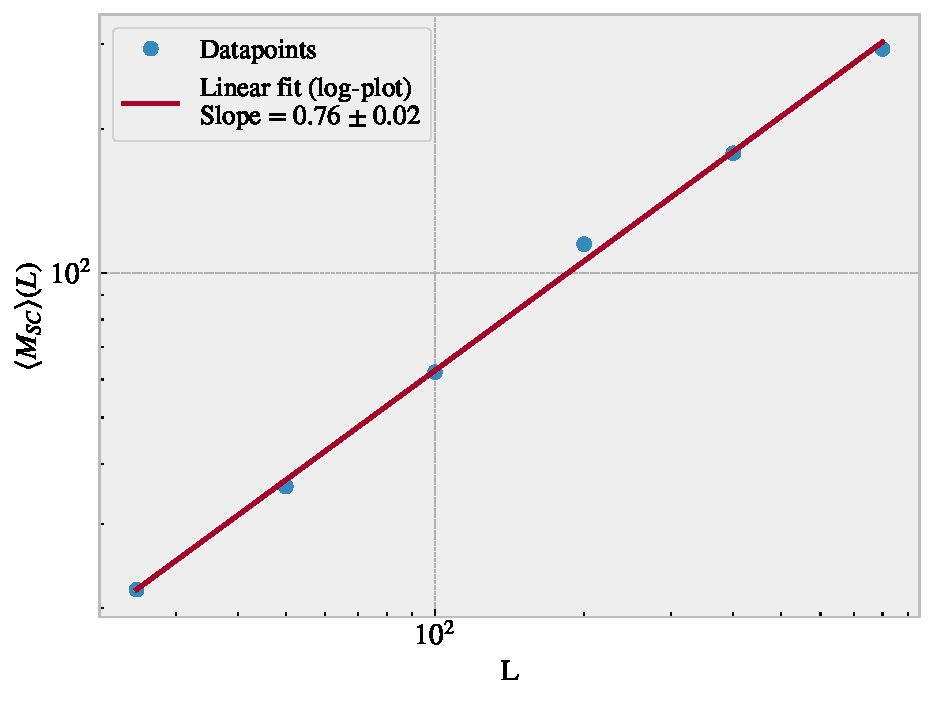
\includegraphics[width=\linewidth]{figures/q.pdf}
  \caption{Mass of connected sites $M_{SC}$ for random walkers on the spanning cluster at $p = p_c$ as a function og $L$. We used $L = 25,50,100,200,400,800$ with 100 Monte Carlo cycles}
  \label{fig:q}
\end{figure}
From figure \ref{fig:q} we estimate
\begin{align*}
  D_{SC} = 0.76 \pm 0.02
\end{align*}
The given value for $D_{SC}$ according to \cite{textbook} is $D_{SC} = 3/4$ giving a relative error
\begin{align*}
  \eta_{D_{SC}}= \left|\frac{0.75 - 0.76}{0.75}\right| = 0.01
\end{align*}



\clearpage
\begin{thebibliography}{9}
  \bibitem{textbook} A.M. Sørensen, 2020, Percolation theory using Python, 20/04/2020, Department of Physics, University of Oslo. Availiable from: \url{https://www.uio.no/studier/emner/matnat/fys/FYS4460/v21/notes/book.pdf}
\end{thebibliography}

\end{document}
